% Turabian Formatting for Theses and Dissertations, 2018/08/06
%
% Developed using the turabian-formatting package (2018/08/01), available through CTAN: http://www.ctan.org/pkg/turabian-formatting
%
% Additional document class formatting options:
%
% raggedright: ragged right formatting without hyphenations
% authordate: support for the author-date citation style
% endnotes: support for endnotes


\documentclass[12pt]{turabian-thesis}

\usepackage{lipsum}
\usepackage{blindtext}

%addbib source file
\addbibresource{backmatter/refferences.bib}

% Information for title page
\title{\MakeTextUppercase{ Template based on Turabian's \emph{A Manual for Writers}, 9th edition}}

%\subtitle{A Template based on Turabian's \emph{A Manual for Writers}, 9th edition}
\author{FIRSTNAME LASTNAME}

\authorinfo{B.S., Georgia Southern University, 2018}
\department{\uppercase{College of [College Name]}}
\institution{Georgia Southern University}
\location{\uppercase{Statesboro, Georgia}}
\degreework{\uppercase{Master of [DegreeWork]}}

%For List of figures and table titles excluded worrd from capitalization 
\Addlcwords{the of into in to a at on and is for}

\makenomenclature

\begin{document}



\frontmatter
\begin{center}
    \MyTitle \\
    by\\
    \MyAuthor \\
    (Under the Direction of Mohammad Abdul Ahad)
\end{center}


\begingroup
\renewcommand{\clearpage}{}
\singlespacing


\chapter*{ABSTRACT}
\vspace*{\stretch{1}} 

\noindent
\lipsum[1-1] 

\vspace*{\stretch{2}}

\noindent
INDEX WORDS: Georgia Southern, Thesis, ETD, Lorem ipsum.
\vspace*{\stretch{4}}

\thispagestyle{empty}
\endgroup




\maketitle
\clearpage
\vspace*{\stretch{1}}

\begin{center}
\textcopyright \space \the\year\par
\MyAuthor \par
All Rights Reserved   
\end{center}

\thispagestyle{empty}
\PrintCommitteeInfoPage{Firstname Lastname}{Firstname Lastname}{Firstname Lastname}{Month of Graduation}

\chapter{DEDICATION}

\begin{center}
	\vspace*{\stretch{1}}
	
	[Optional Text]
	
	\vspace*{\stretch{4}}
\end{center}


\chapter{ACKNOWLEDGEMENTS}
\vspace{\baselineskip}
\doublespacing



\lipsum[4-6]
\tableofcontents 
\listoffigures
\listoftables
\printnomenclature
\mainmatter

\chapter{INTRODUCTION}\label{intro}

\section{First Section}



\lipsum[1-2]

\subsection{A Subsection}



\lipsum[3-4]



\chapter{PROBLEM STATEMENT}


\section{A First Section}

\lipsum[5-7]

\begin{figure}
    \centering
    
\includegraphics[scale=1]{pic/ch1/lion-logo.jpg}
    \caption%
    [\titlecap{A lion logo}]
    {A lion logo}
    \label{fig:lionlogo}
\end{figure}




\subsection{A Subsection}



\lipsum[8-10]\autocite{latexcompanion}


\chapter{FIRST CHAPTER}


\section{Another First Section}



\lipsum[1-2]


\begin{table}[ht]
\renewcommand{\arraystretch}{1.5}
\centering
\caption%
 [\titlecap{This is the sample table caption}]
 {This is the sample table caption.\label{table}}
 \begin{tabular}{||c c c c||}
 
 \hline
 Col1 & Col2 & Col2 & Col3 \\ [0.5ex] 
 \hline\hline
 1 & 6 & 87837 & 787 \\ 
 2 & 7 & 78 & 5415 \\
 3 & 545 & 778 & 7507 \\
 4 & 545 & 18744 & 7560 \\
 5 & 88 & 788 & 6344 \\ [1ex] 
 \hline
 \end{tabular}
\end{table}

\subsection{A Subsection}



\lipsum[3-4]\autocite{einstein}

\chapter{CONCLUSION}\label{chapter conclusion}

Ending of this awesome document. Congratulations, you've made it!\\

\lipsum[5-6]\autocite{knuthwebsite}

\printbibliography[title={REFERENCES}]

\backmatter
    \begin{appendixes}
    

\chapter{FIRST APPENDIX}\label{Appendix 1}

\begin{figure}
    \centering
    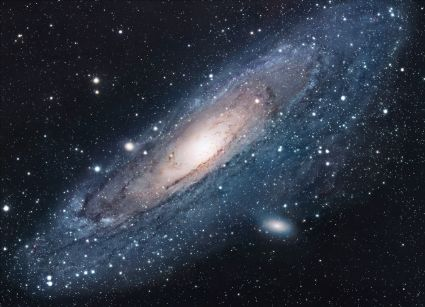
\includegraphics[scale=3]{pic/appendices/universe.jpg}
    \caption%
    [\titlecap{A universe logo}]
    {A universe logo}
    \label{fig:universelogo}
\end{figure}
    \end{appendixes}

    \begin{appendixes}
    
\chapter{{SECOND APPENDIX}}



\begin{table}[h!]
\centering
\begin{tabular}{||c c c c||} 
 \hline
 Col1 & Col2 & Col2 & Col3 \\ [0.5ex] 
 \hline\hline
 1 & 6 & 87837 & 787 \\ 
 2 & 7 & 78 & 5415 \\
 3 & 545 & 778 & 7507 \\
 4 & 545 & 18744 & 7560 \\
 5 & 88 & 788 & 6344 \\ [1ex] 
 \hline
\end{tabular}
\caption
[\titlecap{Table to test captions and labels}]
{Table to test captions and labels}
\label{table:1}
\end{table}


\begin{longtable}[c]{| c | c |}
 \caption{Long table caption.\label{long}}\\

 \hline
 \multicolumn{2}{| c |}{Begin of Table}\\
 \hline
 Something & something else\\
 \hline
 \endfirsthead

 \hline
 \multicolumn{2}{|c|}{Continuation of Table \ref{long}}\\
 \hline
 Something & something else\\
 \hline
 \endhead

 \hline
 \endfoot

 \hline
 \multicolumn{2}{| c |}{End of Table}\\
 \hline\hline
 \endlastfoot

 Lots of lines & like this\\
 Lots of lines & like this\\
 Lots of lines & like this\\
 Lots of lines & like this\\
 Lots of lines & like this\\
 Lots of lines & like this\\
 Lots of lines & like this\\
 Lots of lines & like this\\
 ...
 Lots of lines & like this\\
 \end{longtable}
    \end{appendixes}


\end{document}
